%!TEX root=../thesis.tex
\chapter{A Real-Time model for WebGL} \label{cha:rt_model}

\begin{table}[!htb]
    \centering
    \caption{The test machine hardware specifications.}
    \label{tab:notebook_specs}
    \begin{tabular}{|l|l|l|l|}
    \hline
    \multicolumn{1}{|l|}{\textbf{CPU}} & \multicolumn{1}{l|}{\textbf{GPU}} & \multicolumn{1}{l|}{\textbf{RAM}} & \multicolumn{1}{l|}{\textbf{Hard drive}} \\ \hline
    Intel i7 3537U & Intel® HD Graphics 4000 & 8GB DDR3 & Samsung 850 Evo 250GB \\ \hline
    \end{tabular}
\end{table}

\begin{table}[!htb]
    \centering
    \caption{WebGL functions-to-groups mapping.}
    \label{tab:webgl_func_mapping}
    \begin{tabular}{|l|l|l|}
        \hline
        \textbf{Initialization} & \textbf{Modify data} & \textbf{Display} \\ \hline
        bindBuffer/bindFramebuffer & uniformMatrix3fv/uniformMatrix4fv & drawElements \\
        enable/disable & uniform[1\(\vert\)2\(\vert\)3\(\vert\)4][f\(\vert\)i\(\vert\)iv\(\vert\)fv] & drawArray \\
        viewport & bindTexture/activeTexture &  \\
        clear/clearColor & bufferSubData &  \\
        cullFace &  &  \\
        depthCompare &  &  \\
        useProgram &  &  \\
        colorMask &  &  \\
        \hline
    \end{tabular}
\end{table}

\begin{lstlisting}[caption=Test code caption, language=JavaScript]
    function test(foo, bar) {
        console.log(`foo=${foo}, bar=${bar}`);
    }
\end{lstlisting}

\begin{figure}[!htb]
    \center{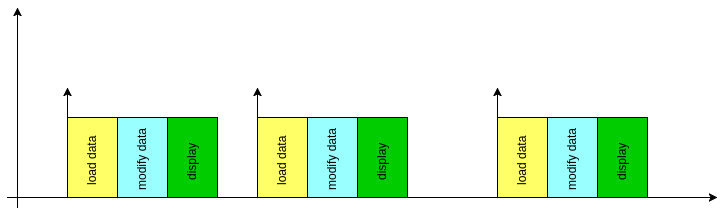
\includegraphics[width=0.6\linewidth]{call_arrival.png}}
    \caption{The function calls arrival approximate model with different groups.}
    \label{img:call_arrival}
\end{figure}
